\documentclass[a4paper,12pt]{article}
\usepackage[utf8]{inputenc}

% Allow the change of line spacing
\usepackage{setspace}

\usepackage{tabularx}

\usepackage{graphicx}

\usepackage[usenames,dvipsnames,table]{xcolor}

%\usepackage{hyperref}
%\usepackage{breakurl}

%opening
%\title{Trainmining}a
%\author{Grupo de Sistemas Inteligentes \\ Universidad Politécnica de Madrid}




\begin{document}
\newcommand\litem[1]{\item{\bfseries #1 }}
\renewcommand{\arraystretch}{1.5} %Makes tables less crammed

\newcommand\headcell[1]{%
  \multicolumn{1}{c|}{\cellcolor{MidnightBlue}\bfseries\sffamily\textcolor{white}{#1}}
}

%\renewcommand{\abstractname}{Executive Summary}
%\begin{abstract}
%
%\end{abstract}

% Set line spacing to 1.5
\onehalfspacing

% Begin a new titlepage. Tit	lepages have special settings like the absence of page numbers.
\begin{titlepage}
\sffamily
% Set the text of the page to right-aligned until \end{flushright}
\begin{flushright}

% Set the space between right page border and text to 2.5cm
\rightskip=-1cm

% Show an image at this position

\includegraphics[scale=1]{./img/logoGSI.png} 
%\includegraphics[bb=0 0 204 110]{web40logo.png}

% Skip a little space
\bigskip
\bigskip
\bigskip



% Create a title for the document and write it in bold font
\LARGE{\textbf{Deliverable 2. Data Analysis.}}
% Again, do a line break
\linebreak
% Create a subtitle
\large{Detailed insight on available data and first statistic analysis.}

% Skip some space
%\bigskip
%\bigskip
%\bigskip
%\bigskip
\bigskip

% Write in very large letters
\LARGE{Grupo de Sistemas Inteligentes}
\linebreak
\large{Departamento de Ingeniería de Sistemas Telemáticos}
% Do a line break right after the \LARGE{...} text
\linebreak
% Write in large letters
\large{Universidad Politécnica de Madrid.}

% Skip some space
\bigskip
\bigskip
\bigskip
\bigskip
\bigskip
\bigskip

\large{Project Report}

% Skip some space
\bigskip

\normalsize{Madrid, October 2012}

% Skip some space
\bigskip
\bigskip
\bigskip
\bigskip
\bigskip
\bigskip
\bigskip
\bigskip
\bigskip
\bigskip
\bigskip
\bigskip
\bigskip
\bigskip
\bigskip
\bigskip

% Provide some author information
\normalsize{Authors:}
\linebreak
\large{Adrián Pérez Orozco}
\linebreak
\large{Álvaro Carrera Barroso}
\linebreak
\large{Carlos A. Iglesias Fernández}

% End right-alignment at this point
\end{flushright}
% End the title page
\end{titlepage}

%\maketitle

\pagenumbering{roman}
\section*{Executive Summary}
\addcontentsline{toc}{section}{Executive Summary} % si queremos que aparezca en el índice

This document describes the data received by Thales Spain for the development of the project \emph{Trainmining}. The original databases used by Thales' maintenance stations are analysed and their structure is described.

A first analysis on the data is performed from a statistical view, obtaining three different indicators to have a better idea of the information we will work with. First of all, the alarm distribution is analysed by categories already existing in the original maintenance station. From this analysis we can observe a clear predominance of single alarm types in each of the maintenance stations. In second place, we have performed a rough correlation analysis, in order to check if correlation of alarm types during a day is consistent between the different stations. We found this correlation to be different, which can be due to difference between systems installed in the different maintenance station. Finally, we have analysed whether the occurrence of certain alarm types varies or not throughout a day. We have found significant differences between occurrence in different time periods, which can be explained due to maintenance procedures happening during certain times during the day.

Finally, the document describes the steps which have been necessary to perform prior to applying data mining algorithms. First of all, data preprocessing has been needed in order to reduce the number of variables which identify each alarm, from the original complex database structure to a reduced representation containing only three variables: \emph{what}, \emph{when} and \emph{where}. To finish, we have also had to transform the data from a continuous log format to discrete observations, as required by the analysis methods we will use in future steps.


\newpage
\tableofcontents % indice de contenidos
\addcontentsline{toc}{section}{Contents} % para que aparezca en el indice de 
\cleardoublepage
\addcontentsline{toc}{section}{List of Figures} % para que aparezca en el indice de contenidos
\listoffigures % indice de figuras

\cleardoublepage
\addcontentsline{toc}{section}{List of tables} % para que aparezca en el indice de contenidos
\listoftables % indice de tablas
\cleardoublepage

\setcounter{page}{1}
\pagenumbering{arabic}

\section{Database description}\label{sec:database_description}
In order to properly process the data provided in form of database backups, it is of essential importance that we completely understand how data is represented in databases. We will analyse the structure and how data is represented in the provided databases: Antequera, Segovia and Sevilla. Each of these database corresponds to a single \emph{maintenance station}, which comprises a whole railway line with several elements along it. The elements with diagnosis systems which can raise alarms are called \emph{installations}, and have different sets of sensors and other systems to control \emph{field elements}. An schematic representation of this architecture is represented in figure~\ref{fig:arch_stations}. The detailed description of available systems and subsystems is of few interest to us. Initially we will only need to differentiate between maintenance stations and installations.

\begin{figure}[hbt]
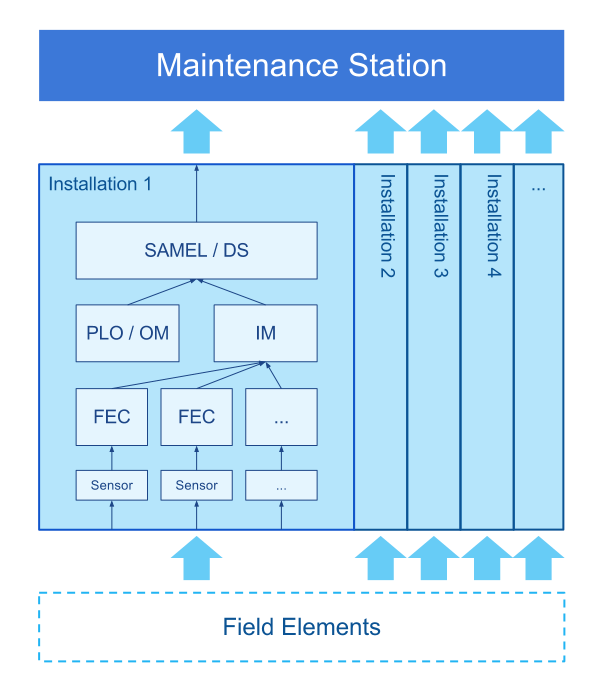
\includegraphics[width=\textwidth]{./img/arch_stations.png}
\caption{Simplified diagram of the maintenance systems architecture} \label{fig:arch_stations}
\end{figure}

Each \emph{maintenance station} has its own unique database, which is of great convenience in order to treat different stations independently. We will start analysing the structure of the main tables of said databases. Due to the high complexity of the maintenance stations, there are a vast amount of tables with configuration parameters and other operational values which are not of interest for our purposes. With assistance from Thales engineers, we have reduced the tables only to those which characterise registered alarms. A total of 4 different tables is used in order to register this information, which are the following:

\begin{description}
\item[Table ER\_ERRORS] This table contains an entry for every alarm received by the maintenance station. Its fields are detailed on table~\ref{tab:table_er_errors}.
\item[Table IG\_INSTALLATIONGENERAL] This table contains information on all the installations managed by the maintenance station. Its fields are detailed on table~\ref{tab:table_ig_installationgeneral}
\item[Table IG\_NODO\_INSTALLATION] This table gathers additional information on installations which are nodes. Nodes are installations which can raise alarms but need a parent installation to send them to the maintenance station. Its fields are detailed on table~\ref{tab:table_ig_nodo_installation}
\item[ERS\_ERRORS\_SAM\_ENCE] This table contains detailed information about the alarms. Its fields are detailed on table~\ref{tab:table_ers_errors_sam_ence}
\item[ERH\_ERRORS\_HSL1] This table is equivalent to ERS\_ERRORS\_SAM\_ENCE. Maintenance stations use one or the other depending on how they receive the alarms. Its only difference with ERS\_ERRORS\_SAM\_ENCE is that registers the method used to receive the alarm. For our purposes it will be treated exactly as its equivalent, and therefore its structure can also be reviewed in table~\ref{tab:table_ers_errors_sam_ence}
\end{description}

Concluding, for each alarm we will have a timestamp and an alarm identifier in table ER\_ERRORS. Alarm identifier is a foreign key which points to table ERS\_ERRORS\_SAM\_ENCE (or equivalent) in which further details of the alarm are saved. Among these details, we can find an installation identifier which specifies which installation has produced the alarm. That identifier is also a foreign key pointing to table DVNI\_INSTALLATIONCODE, in which further details about the installation are stored. Further details on all the database fields are given in tables~\ref{tab:table_er_errors}, \ref{tab:table_ig_installationgeneral}, \ref{tab:table_ig_nodo_installation} and \ref{tab:table_ers_errors_sam_ence}.


\begin{table}
\begin{tabularx}{\textwidth}{|l|X|}
 \hline \headcell{Field name} & \headcell{Description} \\
 \hline
 \hline DVNI\_ERRORNUMBER & Alarm identifier \\
 \hline DVNS\_ERRORTIME & Time-stamp for the alarm \\
 \hline DVNI\_INSTALLATIONCODE & Code of the installation in which the alarm was raised \\
 \hline DVNI\_SENDERINSTALLATIONCODE & Code of the installation from which the alarm was sent (might be different from the one which raised it) \\
 \hline
\end{tabularx}
\caption{Detail of fields on table ER\_ERRORS} \label{tab:table_er_errors}
\end{table}

\begin{table}
\begin{tabularx}{\textwidth}{|l|X|}
 \hline \headcell{Field name} & \headcell{Description} \\
 \hline
 \hline DVNI\_INSTALLATIONCODE & Installation identifier  \\
 \hline DVNI\_SYSTEMCODE & Type of system, as defined in the ``SG\_SYSTEMSGENERAL'' table \\ 
 \hline DVNI\_VERSION & System version \\
 \hline DVAC\_SHORTNAME & Short name of the installation \\
 \hline DVAC\_INSTALLATIONNAME & Name of the installation \\
 \hline DVAC\_LOCATION & Location for the installation \\
 \hline CHK\_IS\_NODE & Whether it is a node (doesn't directly send alarms, only raise them) or not \\
 \hline
\end{tabularx}
\caption{Detail of fields on table IG\_INSTALLATIONGENERAL} \label{tab:table_ig_installationgeneral}
\end{table}

\begin{table}
\begin{tabularx}{\textwidth}{|l|X|}
 \hline \headcell{Field name} & \headcell{Description} \\
 \hline
 \hline IG\_NODO\_INSTALLATION & Identifier of the installation which is a node \\
 \hline DVNI\_FATHER\_INSTALLATION & Identifier of the parent installation \\
 \hline
\end{tabularx}
\caption{Detail of fields on table IG\_NODO\_INSTALLATION} \label{tab:table_ig_nodo_installation}
\end{table}

\begin{table}
\begin{tabularx}{\textwidth}{|l|X|}
 \hline \headcell{Field name} & \headcell{Description} \\
 \hline
 \hline DVNI\_ERRORNUMBER & Alarm identifier \\
 \hline MESSAGE\_ID & Unique alarm identifier \\
 \hline MESSAGE\_TYPE & Type of alarm, always set as ``notification'' (not relevant) \\
 \hline INVOKE\_TYPE & Tells whether the alarm has generated itself due to a connection or disconnection (if type is ``node'') or is generated by a diagnosis system (``saml'') or energy system (``energy'') \\
 \hline INVOKE\_NAME & Irrelevant, always set to ``diagnosis'' \\
 \hline EVENT\_TYPE & Defines the type of alarm which has been generated. Its possible values are listed in table~\ref{tab:field_event_type}. \\
 \hline ADDITIONAL\_TEXT & Alarm code \\
 \hline ADDITIONAL\_INFOS & Additional parameters to be shown in error message \\
 \hline DVNI\_ERRORCATEGORY & Alarm severity. Values from 1 to 5 indicating importance of the alarm, or -1 if the alarm indicates recovery from a previous failure. \\
 \hline
\end{tabularx}
\caption{Detail of fields on table ERS\_ERRORS\_SAM\_ENCE} \label{tab:table_ers_errors_sam_ence}
\end{table}

\begin{table}
\begin{tabularx}{\textwidth}{|l|X|}
  \hline \headcell{Event type} & \headcell{Description} \\
  \hline
  \hline fieldElementAlarm & Alarm related to a field element \\
  \hline fieldElementFailure & Failure in a field element \\
  \hline operatorInformation & Information to the operator \\
  \hline imCpuAndCommunications & Related to IM CPU or IM communications \\
  \hline internalDiagnosis & Internal diagnosis of a system \\
  \hline operationsDiagnosisCommunications & Communication error in Operation and Diagnosis systems \\
  \hline ImFecVersions & IM or FEC version \\
  \hline internalTraces & Internal traces of a system \\
  \hline operatorCommandAnswer & Answer to an operator command \\
  \hline CommProblem & Undefined communication problem \\
  \hline Information & Information message: versions, etc. \\
  \hline CommunicationsAlarm & Procedures and processes to carry information from one point to other \\
  \hline QualityOfServiceAlarm & Loss of quality of service \\
  \hline ProcessingErrorAlarm & SW or processing error \\
  \hline EquipmentAlarm & Equipment failure \\
  \hline EnvironmentAlarm & Related to the environment where the system is located \\
  \hline other & Other \\
  \hline
\end{tabularx}
\caption{Description of values for the field EVENT\_TYPE} \label{tab:field_event_type}
\end{table}
\clearpage
\section{Reduced representation of alarms}\label{sec:reduced_alarms}
In section~\ref{sec:database_description} we have seen a deep definition of all the tables characterising registered alarms. Each of these tables contain several fields, which in total makes an inconvenient large number of variables. While all of them are necessary for correct system function and maintenance purposes, not all of them will be necessary for us to work with alarms.

In order to characterise an event, the main things we need to know can be reduced to three variables:
\begin{itemize}
\item What has happened
\item When has it happened
\item Where has it happened
\end{itemize}

In section~\ref{sec:database_description} we have seen other variables which can provide additional information which - although not essential - can be useful. Specifically, we think the following data can be of possible interest:

\begin{itemize}
\item How severe the event is (severity)
\item Which type of event has happened (event type)
\end{itemize}

These variables can help us to classify alarms or give more importance to those which are more severe. As this information is already provided on given databases, we will keep it and use it for better alarm classification and filtering. However, none of them are essential in order to characterise alarms, as both of them give information which is already implicit in our previous \emph{``what has happened''} variable. Specifically, this information will be of great help in order to make a preliminary statistical insight on the events of the databases, for which a generalisation in terms of severity and category can help us have a better overview of the situation.

We have to identify which fields on our database corresponds to each of the variables we want to obtain. A direct relation is not possible, as details on \emph{what} has happened is registered in several fields of the database. This is necessary for maintenance purposes and better alarm handling in the maintenance station, but for our purposes we should identify \emph{what} has happened with a single variable.

In our database, we have unique alarm identifiers for each of the alarms. For better handling and understanding of what is happening, we will use the textual identifier of the events to identify them. This identifier is gathered on the \emph{ADDITIONAL\_TEXT} field, and can be translated to a full comprehensive human-readable message by the maintenance station. Furthermore, there is additional data to fill in details about the message. For example, we can have an alarm such as ``Communication channel with \emph{X} down'', being \emph{X} an additional parameter saved in the \emph{ADDITIONAL\_INFOS} field. Here we can follow two different approaches: disregard the information about \emph{X}, and just treat it as a ``Channel down'' error; or easily build a compact representation including both variables, such as ``channel.down/x''.

\section{Statistic analysis}
In order to obtain a first general insight of what has happened during the time comprised by our backup data, we will perform a high-level preliminary statistic analysis. In order to achieve a qualitative idea of the type of events, we will use the additional variables we mentioned in section~\ref{sec:reduced_alarms}: severity and event type. These variables provide an already given alarm classification of interest for maintenance operators.

For this purpose, the R language provides a large amount of useful tools which can handle large amounts of data in a very efficient way\cite{quick2010statistical}.

\subsection{Event type distribution}
The first analysis we will perform consists on checking which event types appear in each maintenance station, and which percentage of the total amount of alarms corresponds to each of them. This will help us understand the nature of the events which are usually happening on our railway line.

First of all we will obtain a list of all the types found in each of the stations. We already described in table~\ref{tab:field_event_type} all the possible values for this field, but depending on the diagnosis systems installed on each of the stations, a different subset of them will be used. The list of events for each of the stations is given in tables \ref{tab:field_event_type_antequera} (Antequera), \ref{tab:field_event_type_sevilla} (Sevilla) and \ref{tab:field_event_type_segovia} (Segovia).

\begin{table}
\begin{tabularx}{\textwidth}{|l|X|}
  \hline \headcell{Event type} & \headcell{Description} \\
  \hline
  \hline fieldElementAlarm & Alarm related to a field element \\
  \hline fieldElementFailure & Failure in a field element \\
  \hline operatorInformation & Information to the operator \\
  \hline imCpuAndCommunications & Related to IM CPU or IM communications \\
  \hline internalDiagnosis & Internal diagnosis of a system \\
  \hline operationsDiagnosisCommunications & Communication error in Operation and Diagnosis systems \\
  \hline CommunicationsAlarm & Procedures and processes to carry information from one point to other \\
  \hline
\end{tabularx}
\caption{Event types found in Antequera} \label{tab:field_event_type_antequera}
\end{table}

\begin{table}
\begin{tabularx}{\textwidth}{|l|X|}
  \hline \headcell{Event type} & \headcell{Description} \\
  \hline
  \hline fieldElementAlarm & Alarm related to a field element \\
  \hline fieldElementFailure & Failure in a field element \\
  \hline operatorInformation & Information to the operator \\
  \hline imCpuAndCommunications & Related to IM CPU or IM communications \\
  \hline internalDiagnosis & Internal diagnosis of a system \\
  \hline operationsDiagnosisCommunications & Communication error in Operation and Diagnosis systems \\
  \hline CommunicationsAlarm & Procedures and processes to carry information from one point to other \\
  \hline Other & other \\
  \hline
\end{tabularx}
\caption{Event types found in Sevilla} \label{tab:field_event_type_sevilla}
\end{table}


\begin{table}
\begin{tabularx}{\textwidth}{|l|X|}
  \hline \headcell{Event type} & \headcell{Description} \\
  \hline
  \hline CommProblem & Undefined communication problem \\
  \hline Information & Information message: versions, etc. \\
  \hline CommunicationsAlarm & Procedures and processes to carry information from one point to other \\
  \hline ProcessingErrorAlarm & SW or processing error \\
  \hline EquipmentAlarm & Equipment failure \\
  \hline EnvironmentAlarm & Related to the environment where the system is located \\
  \hline
\end{tabularx}
\caption{Event types found in Segovia} \label{tab:field_event_type_segovia}
\end{table}

From these tables we can observe that alarm types in Antequera and Sevilla are the same (except for unclassified alarms in Sevilla marked as ``other''). From this we can infer that diagnosis systems in these two stations are the same or very similar, as confirmed by Thales' engineers. Segovia however presents a different - although also expectedly similar - set of alarm categories. This is an indicator of diagnosis systems being very different in Segovia than in the other two stations, as confirmed by Thales' engineers.

For better overview of distribution of these alarm types, we will create charts of their respective percentages for each of the stations. These charts can be seen in figures \ref{fig:antequera_chart} (Antequera), \ref{fig:segovia_chart} (Segovia) and \ref{fig:sevilla_chart} (Sevilla).

\begin{figure}[htb]
 \centering
 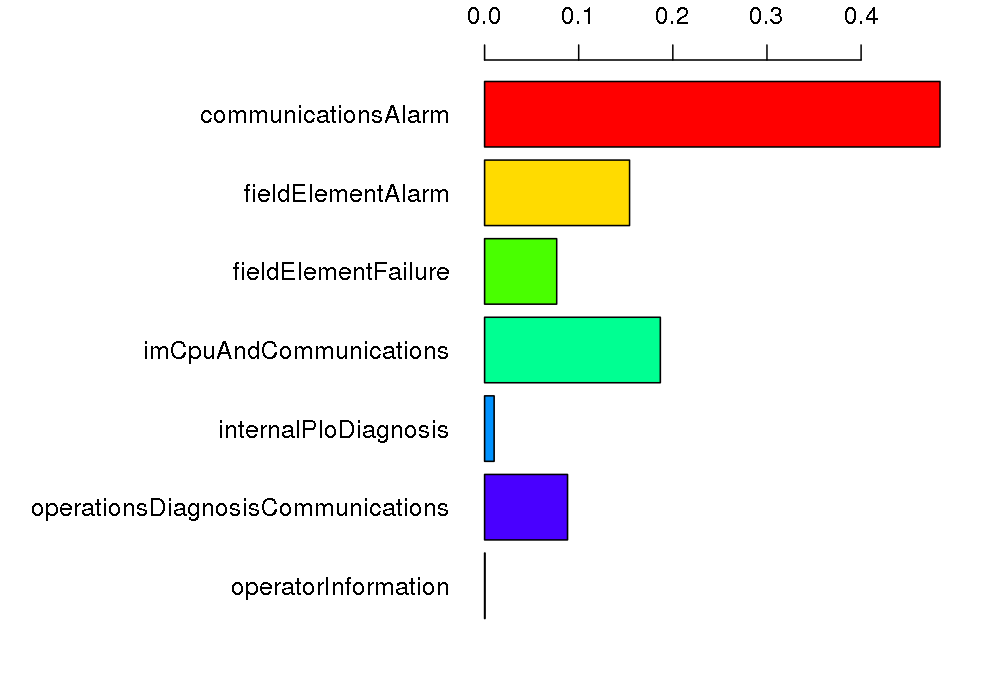
\includegraphics[width=\textwidth]{./img/antequera_graph.png}
 \caption{Alarm information for Antequera}
 \label{fig:antequera_chart}
\end{figure}
\begin{figure}[htb]
 \centering
 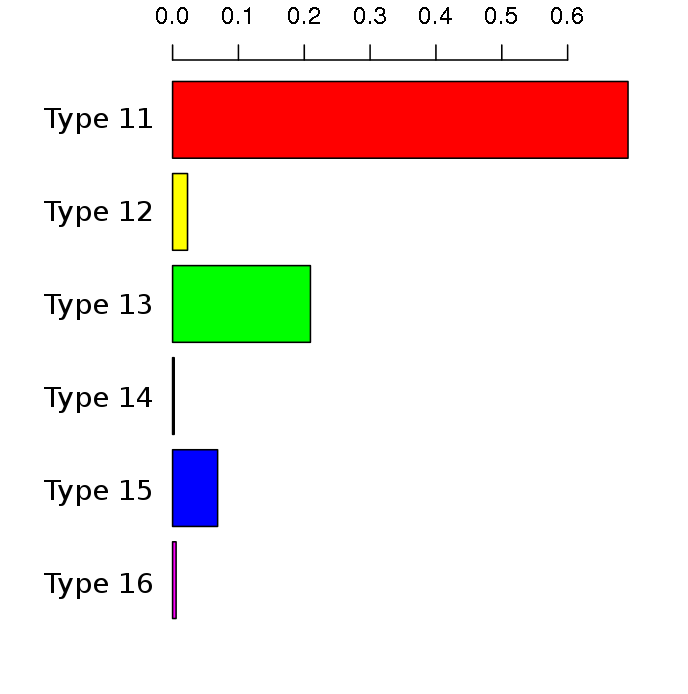
\includegraphics[width=\textwidth]{./img/segovia_graph.png}
 \caption{Alarm information for Segovia}
 \label{fig:segovia_chart}
\end{figure}
\begin{figure}[htb]
 \centering
 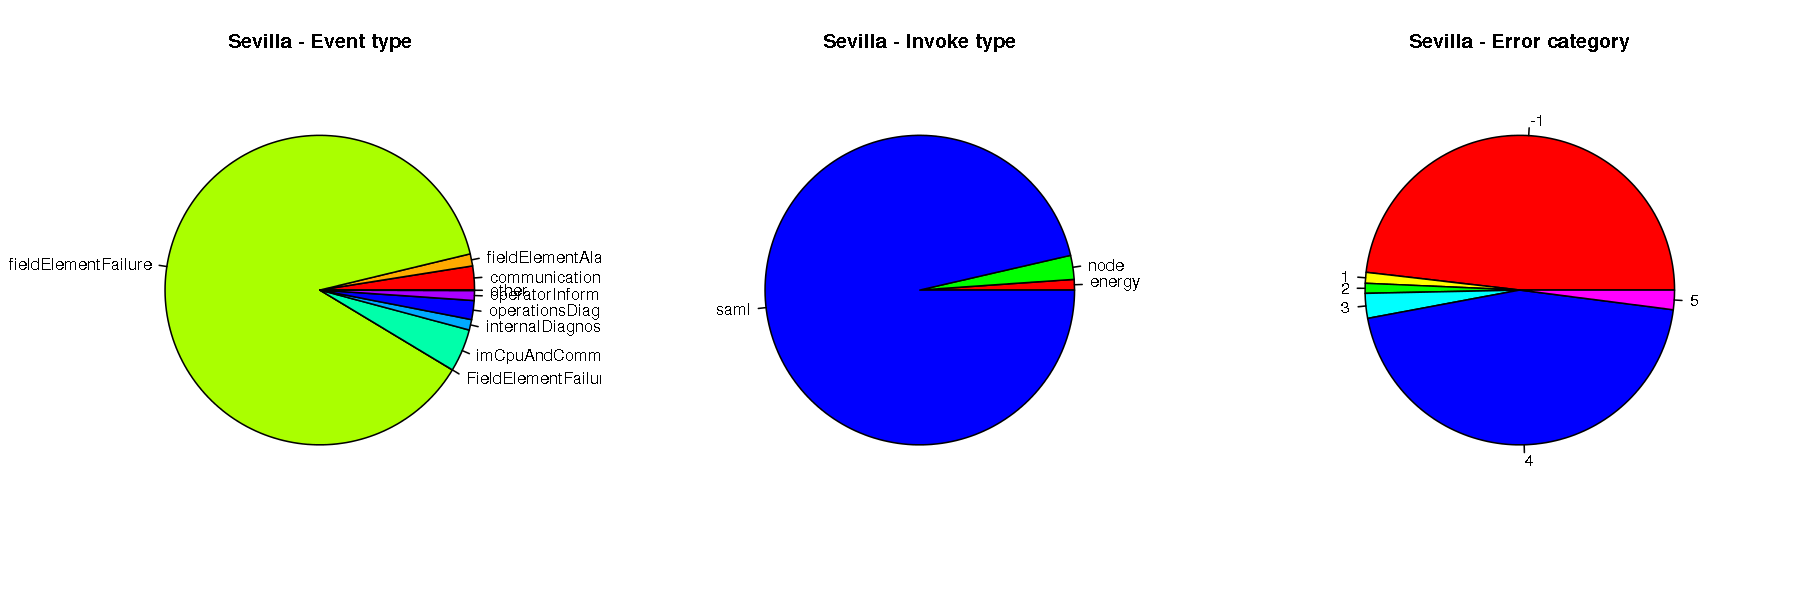
\includegraphics[width=\textwidth]{./img/sevilla_graph.png}
 \caption{Alarm information for Sevilla}
 \label{fig:sevilla_chart}
\end{figure}

\clearpage

We can see that in all of the stations, a single alarm type predominates among all of them. Specifically, we have a vast majority of communication alarms in Antequera and Segovia, and a majority of field element failure alarms in Sevilla. This is not surprising due to the considerable differences between all of them, but can become a problem as the other categories may be too small compared to these main ones when performing Data Mining techniques, obtaining less information - or none at all - from them.

In this direction, it is possible that further actions are required in order to compensate these differences, and avoid that more frequent alarms overshadow the less frequent ones.

\subsection{Daily correlation}
In order to find further differences or similarities between the different stations, we will observe how alarm types are correlated to each others\cite{edwards1976introduction}. That is, how frequent is to find alarms of two specific types happening together during the same short period. For a first insight, we will analyse correlation during daily observations. This correlation information will not be of immediate help in order to predict alarms, as predicting the most frequent alarm type given some conditions is of very little - if any - help. However, it will give us a first idea on how strongly alarms are related to each others.

The result of this correlation is represented in figures \ref{fig:anteq_corr} (Antequera), \ref{fig:segovia_corr} (Segovia) and \ref{fig:sevilla_corr} (Sevilla).

\begin{figure}[htb]
 \centering
 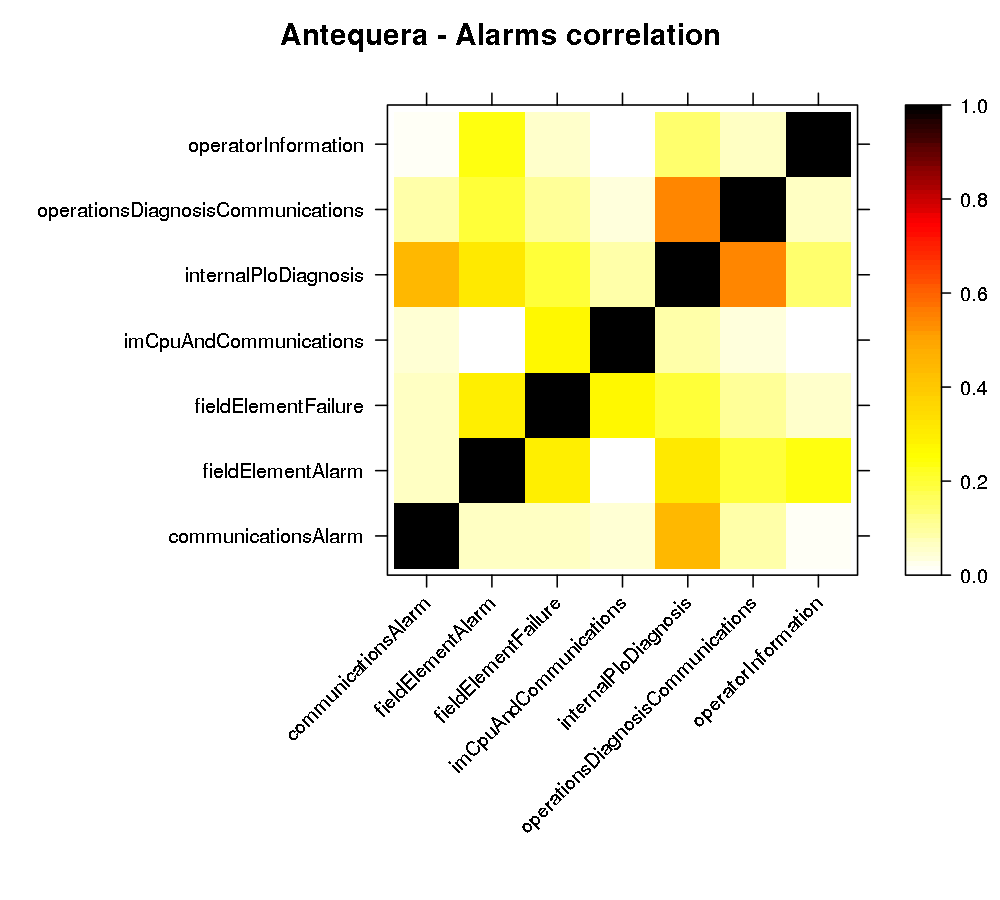
\includegraphics[width=\textwidth]{./img/antequera_corr.png}
 \caption{Daily correlation for Antequera} \label{fig:anteq_corr}
\end{figure}
\begin{figure}[htb]
 \centering
 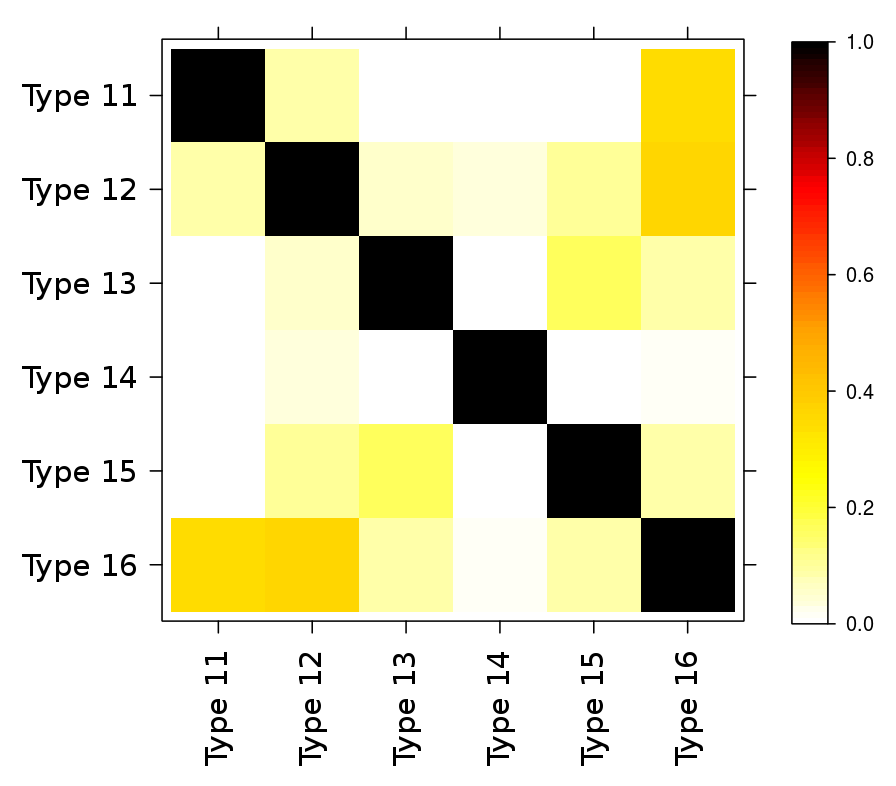
\includegraphics[width=\textwidth]{./img/segovia_corr.png}
 \caption{Daily correlation for Segovia} \label{fig:segovia_corr}
\end{figure}
\begin{figure}[htb]
 \centering
 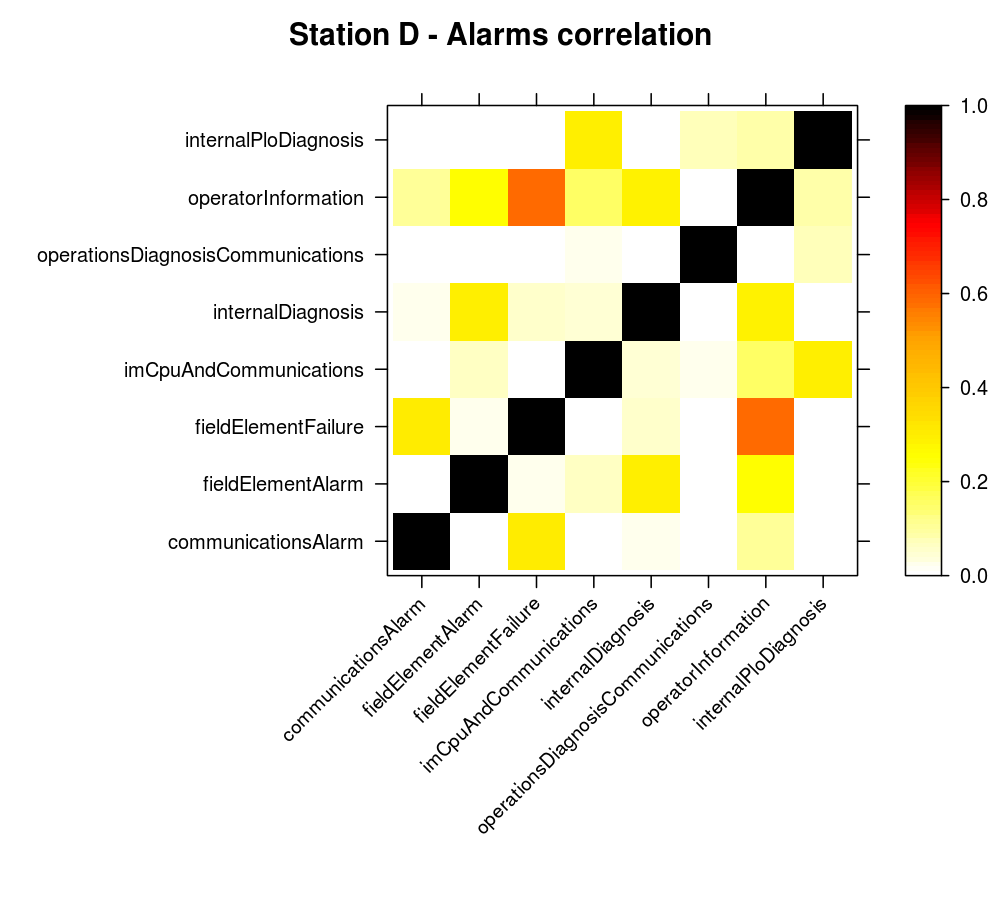
\includegraphics[width=\textwidth]{./img/sevilla_corr.png}
 \caption{Daily correlation for Sevilla} \label{fig:sevilla_corr}
\end{figure}

\clearpage

At first sight, we can affirm that these relations are different even in Sevilla and Antequera, which we found to have similar diagnosis systems. This indicates that, even with similar diagnosis systems, the systems conforming both lines are different. This is indeed confirmed by Thales' engineers, as Antequera station controls a high speed line, while Sevilla corresponds to a commuter line.

Furthermore, we can see strong correlations in Sevilla (Field element failure and operator information) and Segovia (Communications alarms and processing error alarms). As we don't have deep information of the nature of these categories, we can't affirm that this high correlation is due to any causal relation. However, we observe that both these cases show high correlation for the type of alarm which is more frequent in each station, so uneven distribution of alarms might be the cause of this apparent relation between alarms.

From this analysis we can conclude the significant differences in alarm relations between stations, confirming our first thoughts of impossibility of reducing the problem by generalising and merging data from different stations. Further analysis using specific alarm identifiers instead of categories will be needed to obtain relevant results.

\subsection{Hourly timeline}
As an additional first analysis, we wanted to overview the variation of alarm occurrence during the day. During a day, high differences in environment can be experimented which can affect systems in different ways. For instance, temperatures or train affluence can be very different from 4:00 AM to 1:00 PM. These differences can also be found during higher periods, for instance between weekdays and weekends, or between summer time and winter. To start with a specific observation period, we will perform a first analysis between day hours, leaving the other cases for future stages if considered adequate.

Charts with this analysis can be seen in figures \ref{fig:antequera_timeline} (Antequera), \ref{fig:segovia_timeline} (Segovia) and \ref{fig:sevilla_timeline} (Sevilla).

\begin{figure}[htb]
 \centering
 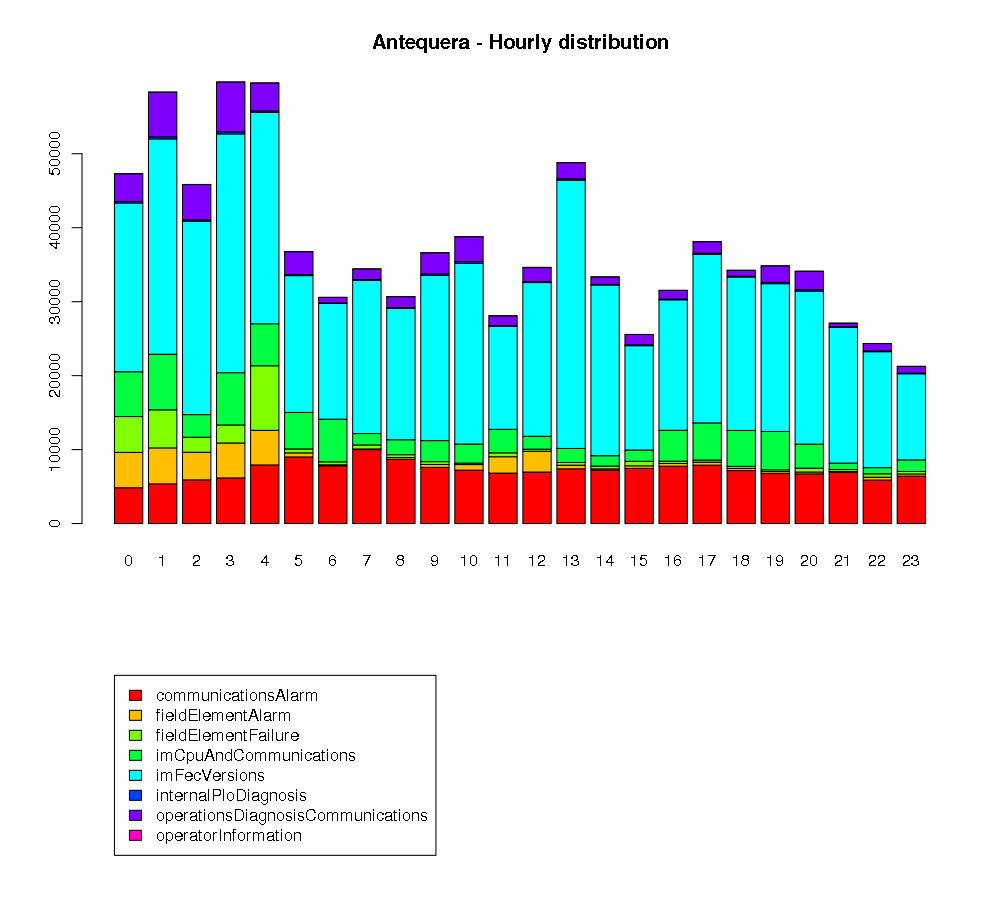
\includegraphics[width=\textwidth]{./img/antequera_timeline.png}
 \caption{Hourly distribution for Antequera (stacked)} \label{fig:antequera_timeline}
\end{figure}
\begin{figure}[htb]
 \centering
 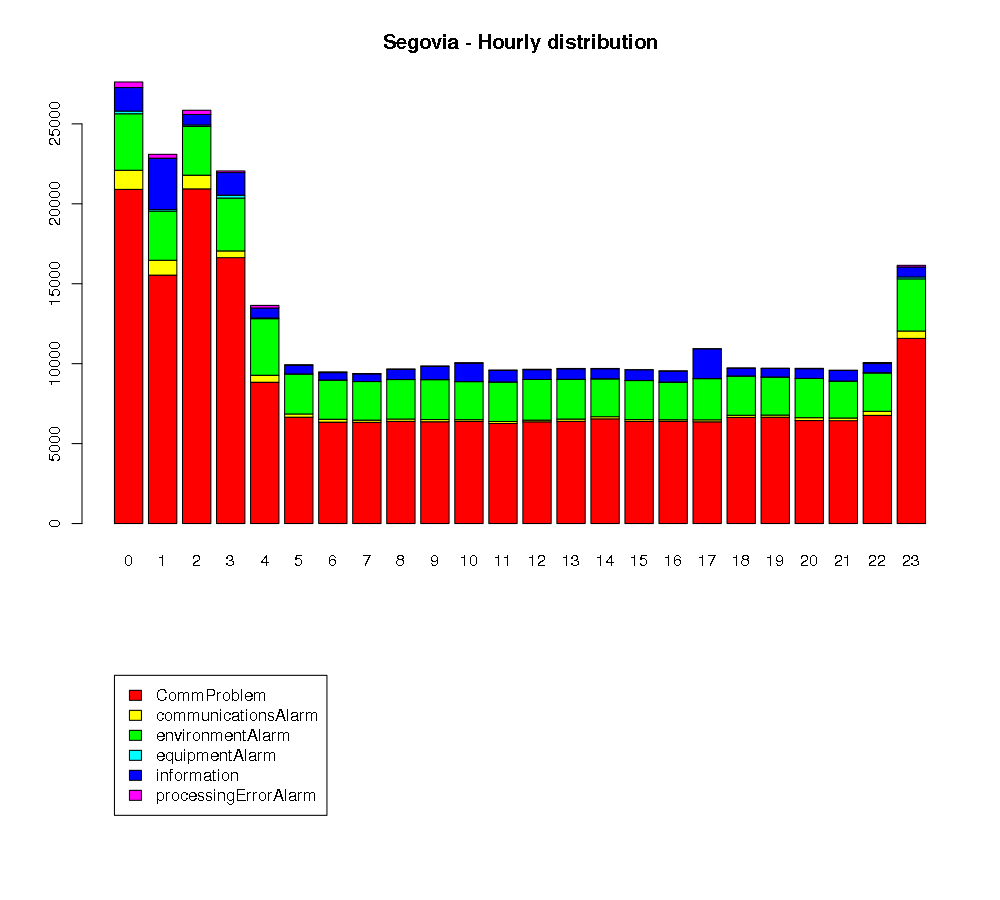
\includegraphics[width=\textwidth]{./img/segovia_timeline.png}
 \caption{Hourly distribution for Segovia (stacked)} \label{fig:segovia_timeline}
\end{figure}
\begin{figure}[htb]
 \centering
 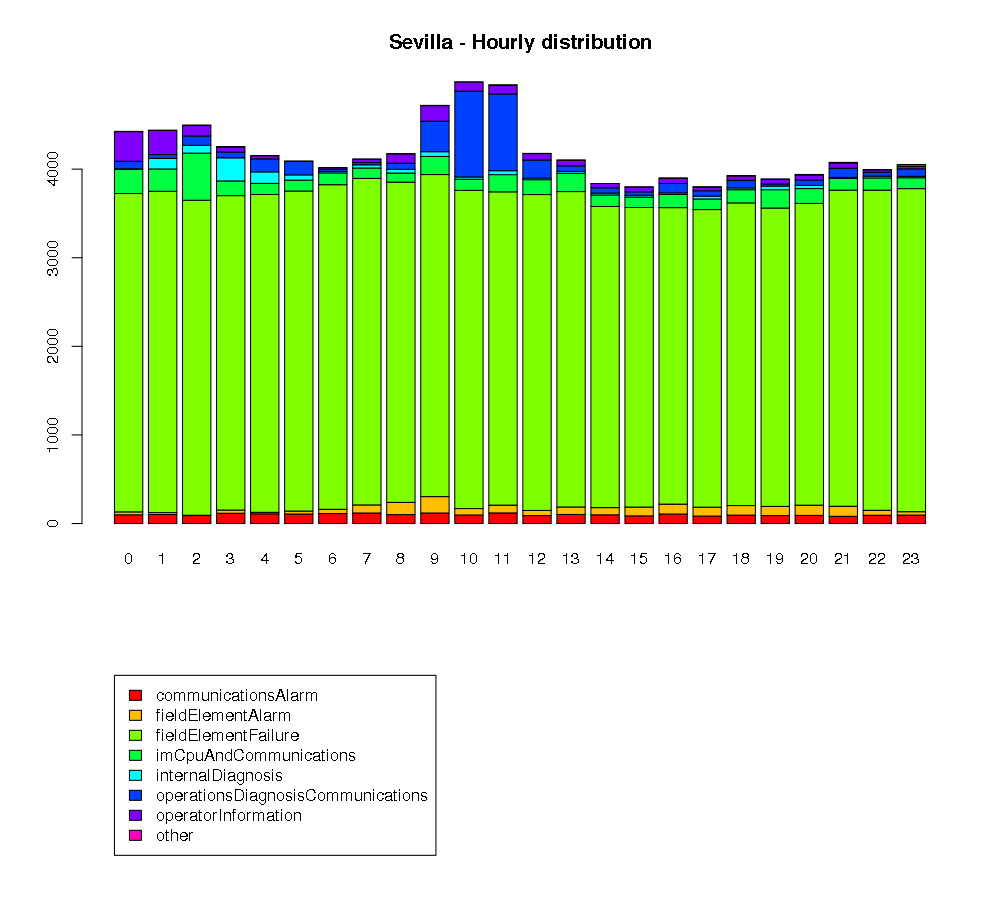
\includegraphics[width=\textwidth]{./img/sevilla_timeline.png}
 \caption{Hourly distribution for Sevilla (stacked)} \label{fig:sevilla_timeline}
\end{figure}

\clearpage

\section{Data preprocessing}\label{sec:data_preprocessing}
As we already mentioned, most data mining processes are usually focused on predicting the value of some variables given the value of the rest variables in a given observation. They work with discrete observations for which each of the variables is analysed or predicted. In our databases we have continuous observations, which need to be transformed into discrete observations\cite{zaki2001spade}.

Depending on the specific application we are using, we can need to transform this data into two possible formats. The first one is the called \emph{basket format}. The most typical example usually used to explain it is a registry of clients of a shop which keeps lists of what the clients buy (hence the name). Therefore, for each observation (often called \emph{transactions} again as an analogy to clients buying in a shop) we will have a list of items happening during that observation (or bought in that transaction). It is important to note that we will keep the same number of variables as in our original data, only that we will stack several items in single entries to obtain discrete observations. It is also important to be careful with which variables we are stacking. While we need to combine all the alarms happening during the same period, it is important not to lose or combine the Installation value. As a result, time identifiers won't be unique in the whole transformed database, but the pair time identifier-installation identifier will.

An example can be seen in tables \ref{tab:data_before_discret} and \ref{tab:basket_example}. Table~\ref{tab:data_before_discret} is an example of the original data, and table~\ref{tab:basket_example} is the equivalent data transformed into basket format.

The second possible transformation is to represent the occurrence of each alarm with an additional variable. This means that we will need as many variables as the total number of possible different alarms in our system. Same as before, we must be careful to preserve data on installations, and create independent observations for each time slot and each installation. Each additional variable can represent the alarms in different ways. Either in a boolean sense (whether the alarms happens at least once or not at all) or the specific number of times the alarm has happened. In order not to lose information at this stage of processing, we will keep the specific amount of times each alarm has happened, which can be easily reduced to a boolean variable if appropriate for the application.

This second case is indeed a more strict representation of the \emph{basket format}. While in basket format we just needed a single variable where we could add all the alarms in the form of a list, here we need to specify exactly the number of times all the variables have happened. Both of them are equivalent and we can easily convert data from one format to another, but as different algorithms will work specifically with one of each forms of representation, it's convenient to perform both transformations from original data and use each one accordingly.

An example of this transformation can be seen in tables \ref{tab:data_before_discret} and \ref{tab:expanded_example}. Table~\ref{tab:data_before_discret} is an example of the original data, and table~\ref{tab:expanded_example} is the equivalent data discretised with additional variables.

These transformations have been automatised with R scripts, in a way so we can easily repeat these processes for different time spans. This will allow us to work at any moment with different time resolutions without any significant additional work for further transformations.

\begin{table}
\begin{center}
\begin{tabular}{|c|c|c|}
\hline \headcell{Timestamp} & \headcell{Installation} & \headcell{Alarm} \\ 
\hline
\hline 01-01-2011 00:00 & 0 & Alarm A \\ 
\hline 01-01-2011 00:30 & 0 & Alarm B \\ 
\hline 01-01-2011 00:45 & 1 & Alarm B \\ 
\hline 01-01-2011 01:10 & 0 & Alarm C \\ 
\hline 01-01-2011 01:20 & 0 & Alarm A \\ 
\hline 01-01-2011 01:22 & 0 & Alarm A \\
\hline 01-01-2011 01:25 & 1 & Alarm C \\ 
\hline 01-01-2011 01:30 & 1 & Alarm A \\ 
\hline 01-01-2011 02:20 & 0 & Alarm A \\ 
\hline 01-01-2011 02:30 & 1 & Alarm A \\ 
\hline 01-01-2011 02:45 & 0 & Alarm B \\ 
\hline ... & ... & ... \\ 
\hline 
\end{tabular} 
\end{center} 
\caption {Continuous observation. Example of alarms in log format.} \label{tab:data_before_discret} 
\end{table}

\begin{table}
\begin{center}
\begin{tabular}{|c|c|c|}
\hline \headcell{Time} & \headcell{Installation} & \headcell{Alarms} \\ 
\hline
\hline 0 & 0 & A, B \\ 
\hline 0 & 1 & B \\ 
\hline 1 & 0 & C, A, A \\ 
\hline 1 & 1 & C, A \\ 
\hline 2 & 0 & A, B \\ 
\hline 2 & 1 & A \\ 
\hline ... & ... & ... \\ 
\hline 
\end{tabular} 
\end{center}
\caption{An example of discretised data in basket format.} \label{tab:basket_example}
\end{table}

\begin{table}
\begin{center}
\begin{tabular}{|c|c|c|c|c|}
\hline \headcell{Time} & \headcell{Installation} & \headcell{Alarm A} & \headcell{Alarm B} & \headcell{Alarm C} \\ 
\hline 
\hline 0 & 0 & 1 & 1 & 0 \\ 
\hline 0 & 1 & 0 & 1 & 0 \\ 
\hline 1 & 0 & 2 & 0 & 1 \\ 
\hline 1 & 1 & 1 & 0 & 1 \\ 
\hline 2 & 0 & 1 & 1 & 0 \\ 
\hline 2 & 1 & 1 & 0 & 0 \\ 
\hline ... & ... & ... & ... & ... \\ 
\hline 
\end{tabular} 
\end{center} 
\caption {Example of discretised data} \label{tab:expanded_example} 
\end{table}

\clearpage

\section{Final comments}
After this step, we have a complete understanding of the database models and how alarms are represented in the provided logs. The preliminary statistic analysis has also provided additional information on the data which will help us to fine-tune actions taken in future steps. 

Furthermore, we are already prepared to load our data into our selected software solutions and start with the \emph{Data Mining} processes. In next steps, we will directly use data in the format here presented as input for already existing data mining solutions, which we will use as starting point for our knowledge discovery process. It is possible that additional transformations are found to be required in further steps of the project, case in which we would have to return to this point and perform whichever process is required by any other algorithm or software.

Specifically, we will continue our work with two solutions: the \emph{cSPADE} algorithm and the \emph{GeNIe/Smile} framework. cSPADE is an implementation of a data mining algorithm which looks for frequent sequences in our database. It needs data in the aforementioned \emph{basket format} - as shown in table~\ref{tab:basket_example} - and will help us obtain association rules to obtain predictions. At the same time, we will work on a relational model using \emph{bayesian networks}, for which we will use the \emph{GeNIe/SMILE} framework. This framework needs the data input to be in the extended format we mentioned in section~\ref{sec:data_preprocessing} and exemplified in table~\ref{tab:expanded_example}.

We have selected an observation time of 24 hours, which will affect the time over which we can make sensible predictions. It is possible that we need to change it to analyse different possibilities, which can be easily done with the R scripts developed in this stage. This will allow comparison of results using different observation spans.

\clearpage

\bibliographystyle{plain} 
\bibliography{datamining}

\end{document}


